\documentclass{report}
\usepackage[utf8]{inputenc}
\usepackage[T1]{fontenc}
\usepackage[italian]{babel}

%Disable all warnings issued by latex starting with "You have..."
\usepackage{silence}
\WarningFilter{latex}{You have requested package}

%Bib
\usepackage[style=numeric]{biblatex}
\addbibresource{references.bib}

\usepackage{csquotes}
%\usepackage{natbib}

%Import
\usepackage{marvosym}
\usepackage{fancyvrb}
\usepackage[usenames]{color}
\usepackage[hidelinks]{hyperref}
\usepackage{url}
\usepackage{graphicx}
\usepackage{xcolor}
\usepackage{amsmath,amsfonts,amssymb,amsthm}
\usepackage{caption}
\usepackage{enumerate}
\usepackage{multicol}
\usepackage{subcaption}
\usepackage{float}
\usepackage{indentfirst}
\usepackage{listings}
\usepackage{tocloft}
\usepackage[most]{tcolorbox}
\usepackage{pgfplots}
\usepackage{style/pgfplotsthemetol}
\pgfplotsset{compat=1.16}
\definecolor{lstgrey}{rgb}{0.94,0.95,1}
\lstset{
    backgroundcolor=\color{lstgrey},
    frame=single,
    rulecolor=\color{lstgrey}, % make frame "invisible"
    captionpos=t,
    tabsize=2,
    numberbychapter=false,
    showstringspaces=false,
    breaklines=true,
}
%LINK CLICCABILI
\hypersetup{
    colorlinks = true,
    linkcolor = .,
    citecolor = {blue},
    linkbordercolor = {white},
    urlcolor = {blue},
}
%TABELLE TBCOLORBOX
\tcbset{
        enhanced,
        colback=red!5!white,
        boxrule=0.1pt,
        colframe=red!75!black,
        fonttitle=\bfseries
       }

\newcommand{\executeiffilenewer}[3]{%
 \ifnum\pdfstrcmp{\pdffilemoddate{#1}}%
 {\pdffilemoddate{#2}}>0%
 {\immediate\write18{#3}}\fi%
}
\newcommand{\includesvg}[1]{%
 \executeiffilenewer{#1.svg}{#1.pdf}%
 {inkscape -z -D --file=#1.svg %
 --export-pdf=#1.pdf --export-latex}%
 \input{#1.tex}%
}

%PATH IMMAGINI
\graphicspath{{images/} {plantuml/rendered/} }
\newcommand{\emailaddr}[1]{\href{mailto:#1}{\texttt{#1}}}

\title{\LARGE
    AKKA RAFT
}

\author{
    Author 1 \\ \emailaddr{sara.kiade@studio.unibo.it}
    \and 
    Author 2 \\ \emailaddr{gyordan.caminati@studio.unibo.it} 
    \and 
    Author 3 \\ \emailaddr{luca.giulianini2@studio.unibo.it}
}

\date{January 2019}

\begin{document}
\maketitle
\tableofcontents

% -*- root: ../main.tex -*-
\begin{abstract}
Il problema del consenso rappresenta un elemento cruciale nei sistemi distribuiti, dove spesso diverse entità si trovano a dover concordare su un valore da assumere, al fine di convergere al medesimo stato. Nello specifico, il problema si presenta nel momento in cui si ha a che fare con \textbf{macchine a stati replicate}, dove la replicazione del dato deve mantenersi \textbf{consistente}.
Per portare a termine questo compito, sono attualmente disponibili diversi algoritmi di consenso.\newline
Il presente progetto consiste nello \textbf{studio approfondito e documentato} dell'algoritmo di consenso \textbf{RAFT} e delle sue applicazioni, arricchito da una implementazione che permette di evidenziare le sue peculiarità e di testarne il comportamento in diverse situazioni. Tale implementazione, infatti, fornisce un interfaccia utente tramite la quale è possibile agire su parametri significativi, al fine di poter eseguire agevolmente dei \textbf{test} e avere un riscontro degli effetti di questi ultimi sul \textbf{comportamento} del sistema.
\end{abstract}
% -*- root: ../main.tex -*-
\chapter{Introduzione}
	Lo sviluppo in ambito ICT avvenuto negli ultimi anni unito alla informatizzazione massiva dei processi ha portato molte aziende a dover ripensare gran parte dei propri sistemi. Questi sistemi, infatti, erano progettati specificatamente per \textbf{environment statici} e a fronte di richieste di grande \textbf{scalabilità} ed elevata \textbf{dinamicità} mostrarono subito le loro debolezze.

	\section{Sistemi Distribuiti}
	Gran parte dei sistemi più complessi al giorno d'oggi sono \textbf{sistemi distribuiti}, ossia sistemi in cui la computazione non avviene in modo \textit{situato} nella medesima macchina nel medesimo processo ma in modo distribuito fra differenti macchine. Il concetto di distribuzione porta ad una computazione che esula dal \textbf{tempo} e dallo \textbf{spazio} nella loro rappresentazione \textbf{assoluta}.
	\begin{itemize}
		\item{\textbf{Tempo:}}
		Esiste solo una concezione di \textbf{tempo logico} ossia un tempo relativo al singolo sistema distribuito. Per fare ciò vengono usate delle astrazioni \textit{logiche} di tempo chiamate: \textbf{vector clocks} \cite[Lamport:1978]{Lamport:1978}.\\
		Vedremo che con l'algoritmo RAFT verrà utilizzata una astrazione simile per il concetto di \texttt{term}.
		\item{\textbf{Spazio:}}
		Un sistema distribuito nella sua forma più semplice consiste di un insieme di macchine interconnesse fra loro che eseguono una \textit{computazione} in modo \textit{coordinato} e \textit{decentralizzato}. Il sistema idealmente dovrebbe \textit{astrarre} dalla distribuzione spaziale delle singole unità che lo compongono.
	\end{itemize}

	\section{Il Teorema CAP}
	Ogni sistema distribuito è caratterizzato da 3 proprietà fondamentali:
	\begin{itemize}
	  	\item{\textbf{Consistency:}}
	  	Vogliamo che un sistema si comporti correttamente, ossia che possa fornire output corretti a fronte di qualsiasi input.
	  	\item{\textbf{Availability:}}
	  	Vogliamo che il sistema sia sempre disponibile.
	  	\item{\textbf{Partition Tolerance:}}
	  	Vogliamo che il sistema sia robusto contro contro partizioni dello stesso e quindi crash di qualsiasi componente.
	  \end{itemize}
	Il teorema \textbf{CAP} afferma che in un qualsiasi sistema distribuito si possono garantire al massimo due proprietà \cite[Brewer:2000]{Brewer:2000}
	Esiste dunque un tradeoff fra \textbf{safety} e \textbf{liveness}.

	\section{Terminologia}
		\paragraph{Safety}
		Il concetto di consistenza richiama fondamentalmente il concetto di safety secondo il quale:\\ ``\emph{Something bad ($\phi$) always not happends}'' 
		\begin{equation}
			\square \lnot \phi
		\end{equation}
		\paragraph{Liveness}
		Il concetto di availability riprende invece quello di liveness secondo cui:\\
		``\emph{Something good ($\psi$) eventually happends}''
		\begin{equation}
			\square \lozenge \psi
		\end{equation}
		\paragraph{Partition Tolerance:}
		Quando un sistema è \textit{partitioned} allora tutti i messaggi scambiati da un nodo in un componente della partizione a un altro nodo della partizione sono persi.
		\paragraph{Componente}
		In un sistema distribuito è formato da vari componenti; ogni componente ha queste caratteristiche:
		\begin{itemize}
		 	\item{\textbf{Indipendenza:}}
		 	Ogni componente è una entità autonoma e indipendente e dunque generalmente disaccoppiata.
		 	\item{\textbf{Eterogeneità:}}
		 	Non sono date \textit{assunzioni} sulla \textbf{natura} delle singole entità sulla loro \textit{struttura} e \textbf{comportamento}
		\end{itemize}
		\paragraph{Coerenza}
		Un sistema distribuito ha come scopo principe quello di rappresentare e gestire in modo coerente i vari componenti con lo scopo di risultare dall'esterno come un sistema omogeneo \emph{Working as One, Looking as One}.\\
		La coerenza viene ottenuta anche attraverso l'utilizzo di un \textbf{Middleware} il quale permette a tutti i componenti di interfacciarsi su un \textit{layer condiviso} che espone la \textit{stessa interfaccia} su architetture e linguaggi diversi.
		\paragraph{Interazione}
		Secondo una definizione più specifica fornita da \cite[Colouris:2012]{Colouris:2012} un sistema distribuito è un sistema in cui componenti collegati in rete comunicano e si coordinano attraverso \textbf{scambio di messaggi}.\\
		L'interazione in questo caso diventa fondamentale per garantire la \textbf{coerenza} e l'\textbf{uniformità} del sistema.

	\section{Replicazione e Fault Tolerance}
	Secondo molti un sistema distribuito porta in generale più complessità e addirittura meno vantaggi rispetto ad un sistema situato. Esistono però alcuni proprietà fondamentali che i sistemi situati, che operano nel concentrato, non riescono a garantire.
		\subsubsection{Replicazione e Consistenza}
		La replicazione porta parecchi benefici fra cui:
		\begin{itemize}
			\item{\textbf{Reliability}}
			Il sistema è molto più reliable dato che esistono repliche che possono essere operative anche a fronte di guasti di altre unità.
			\item{\textbf{Fault Tolerance}}
			Un componente può fallire mentre il resto del sistema continua a funzionare. Abbiamo dunque la resistenza contro \textit{partial failure} nel sistema.
			\item{\textbf{Accessibility}}
			Avendo più repliche a disposizione, si rende più agevole l'accessibilità e il carico può essere bilanciato in modo più semplice.
			\item{\textbf{Performance}}
			Non avendo un solo punto di accesso, anche le performance traggono giovamento.
			\item{\textbf{Scalability}}
			IL sistema è indipendente dal numero di componenti presenti. Questo permette grande \textit{elasticità} nella gestione dei componenti.
		\end{itemize}
		ma anche alcuni problemi che bisognerà arginare:
		\begin{itemize}
			\item{\textbf{Costo}}
			Il costo della replicazione è direttamente correlato al costo delle macchine utilizzate per replicare i dati. Più hardware viene utilizzato più il costo collegato è elevato.
			\item{\textbf{Consistenza}}
			Il problema della consistenza è il problema fondamentale per i sistemi distribuiti. Dato che un sistema multi-replica non garantisce nulla su come e quando verranno replicati i dati, bisogna trovare un modo per garantire che lo stato dei singoli componenti sia consistente con quello del sistema. Questo deve essere fatto anche a discapito di altre proprietà come la \textbf{availability} come già visto nel teorema CAP. 
		\end{itemize}

    \subsubsection{Fault Tolerance}
    Lo scopo fondamentale della fault tolerance è quello di permette al sistema di \textbf{sopravvivere} a e in alcuni casi \textbf{risolvere} autonomamente le \textbf{failures}.
    Generalmente questo comportamento viene ottenuto limitando l'impatto della failure sull'intero sistema cercando di sfruttare i componenti integri al fine di risolvere gli stessi fallimenti.



% -*- root: ../main.tex -*-
\chapter{Consenso e State Machine Replication}
Il principale vantaggio fornito dai sistemi distribuiti rispetto ai sistemi centralizzati sta nel fatto di poter garantire un servizio continuo malgrado \textit{failures} e \textit{malfunzionamenti} \cite[Friedman:1996]{Friedman:1996}.
L'idea infatti è quella di poter realizzare sistemi che possano far fonte a componenti inaffidabili che non possono garantire una disponibilità costante; questi sistemi devono essere in grado di \textit{reagire} e \textit{adattarsi} automaticamente ai cambiamenti.\\
Fra le sfide più importanti che i sistemi distribuiti devono affrontare al giorno d'oggi troviamo: la gestione delle failures, la coordinazione, il discovery di servizi e la gestione della configurazione; tutti problemi difficili da risolvere in ambienti dinamici. Fortunatamente il consenso distribuito permette di risolvere gran parte di questi problemi.
	
	\section{Il problema del Consenso}
	Gli algoritmi di consenso rappresentano gli algoritmi fondamentali e più importanti nell'ambito dei sistemi distribuiti.
	Gli algoritmi di consenso permettono a una collezione di \textbf{macchine eterogenee} di lavorare in qualche modo come se fossero un \textbf{una sola macchina}.\\
	Si parte dunque con un insieme di \textbf{macchine} singolarmente \textbf{inaffidabili} e si fa in modo che esse si comportino come un'\textbf{unica macchina super-affidabile} che garantisce di operare in modo reliable anche nel caso in cui alcune macchine falliscano.\\
	All'interno di un gruppo di consenso (\textbf{consensus group}) i fallimenti sono gestiti in un modo studiato e comprovato, questo permette di avere un \textit{modello di funzionamento} robusto e affidabile.\\
	Data l'estremam \textbf{availability} e \textbf{raliability} dei consensus group, altri sistemi possono decidere di usare un consensus group come fondamenta per garantire fault tolerance; questo porta gli algoritmi di consenso a giocano un ruolo fondamentale nella costruzione di sistemi reliable di grandi dimensioni. 

	\section{Replicated State Machine}
	Gli algoritmi di consenso sono generalmente utilizzati nel contesto di quelle che chiamiamo replicated state machines. Prima di parlare di macchine a stati replicate bisogna definire cos'è una macchina a stati.\\
	Una macchina a stati è generalmente un programma che: 
	\begin{itemize}
		\item{\textit{accetta e risponde} a vari tipi di interazioni o \textbf{stimoli esterni}.}
		\item{Gli stimoli possono essere nella forma di \textit{comandi} che provengono da clients e hanno lo scopo di gestire lo \textbf{stato interno} della macchina.}
	\end{itemize}
	Al giorno d'oggi le state machine rappresentano un modello generale di computazione estremamente diffuso. Gran parte dei sistemi a larga scala (as-a-service) che utilizziamo solitamente sono nella forma di macchine a stati.

	\begin{figure}[H]
		\centering
		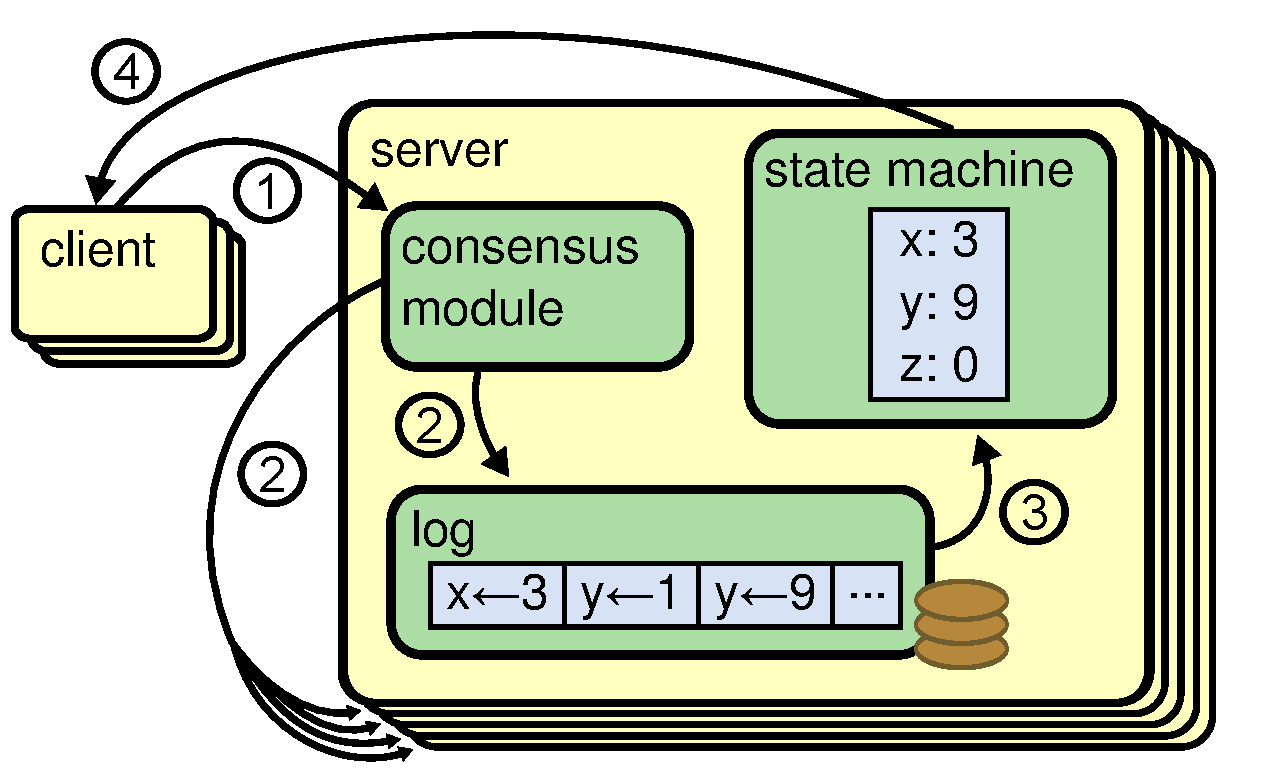
\includegraphics[width=0.99\columnwidth]{statemachine}
		\caption{Un modello di state machine semplificato}
		\label{fig:figure1}
	\end{figure}  
 % -*- root: ../main.tex -*-
\chapter{RAFT}
	
	\section{L'algoritmo PAXOS}
	\section{L'algoritmo RAFT}
		\subsection{Leader Election}
		\subsection{Normal Operation}
		\subsection{Safety e Consistency}
		\subsection{Neutralize Old Leaders}
		\subsection{Client Protocol}
		\subsection{Configuration Changes}
% -*- root: ../main.tex -*-
\chapter{RAFT: Implementazione}
	Dopo aver appreso in maniera approfondita le dinamiche dell'algoritmo RAFT, si è passati alle fasi di progettazione, sviluppo e testing di un applicativo che ne implementi il funzionamento. 
\section{Goal/Requirements}

Detailed description of the project goals, requirements, and expected outcomes.
%
Use case Diagrams, examples, or Q/A simulations are welcome.

\subsection{Scenarios}

Informal description of the ways users are expected to interact with your project.
%
It should describe \emph{how} and \emph{why} a user should use / interact with the system.

\subsection{Self-assessment policy}

\begin{itemize}
    \item How should the \emph{quality} of the \emph{produced software} be assessed?
    
    \item How should the \emph{effectiveness} of the project outcomes be assessed?
\end{itemize}
% -*- root: ../../main.tex -*-               
\section{Analisi dei Requisiti}
L'applicativo è una rappresentazione operativa di RAFT; per questo motivo, i dettagli dei requisiti che deve avere sono insiti nelle caratteristiche dell'algoritmo discusse in precedenza. 

Il sistema dovrà consistere in un insieme di nodi che rappresentano due entità principali:
	\begin{itemize}
		\item \textbf{Un client:} si occupa di inoltrare le richieste ai server e ricevere gli esiti.
		\item \textbf{$n$ server:} accolgono le richieste del client, le eseguono e comunicano il risultato. Ognuna di queste entità, in un dato istante, ricopre uno e un solo ruolo tra \textit{Leader, Candidate} e \textit{Follower}
	\end{itemize}

Dal momento che queste entità devono essere \textbf{indipendenti} ed interagire tra loro, si è scelto di utilizzare il \textbf{paradigma ad attori}, che rende possibile agire ad un livello di astrazione molto elevato permettendo di facilitare la gestione delle dinamiche di interazione.


	\subsection{Il paradigma ad attori} \label{Actors}
	Si tratta di un paradigma nato per riuscire a sfruttare al meglio le potenzialità della programmazione ad \textbf{oggetti} in ambito \textbf{concorrente}, interamente basato sul concetto di \textbf{attore}: \emph{everything is an actor}.

	Per \textbf{attore} si intende un' entità indipendente, univocamente identificata, caratterizzata dai seguenti elementi:
	\begin{itemize}
		\item \emph{Una mailbox, alla quale arrivano messaggi provenienti da altri attori.}
		\item \emph{Uno \textbf{stato}, non accessibile dall'esterno.}
		\item \emph{Un \textbf{comportamento} (behaviour), che definisce il modo in cui l'attore reagisce ai messaggi ricevuti.}
		\item \emph{Un \textbf{flusso di controllo} indipendente.}
	\end{itemize}

	Per rendere possibile la realizzazione di un sistema ad attori, sono necessarie tre primitive:
	\begin{itemize}
		\item \textbf{Send:} per inviare un messaggio ad un altro attore, compreso il mittente.
		\item \textbf{Create:} per creare un attore figlio.
		\item \textbf{Become:} per cambiare il comportamento dell'attore. Ogni comportamento è caratterizzato da una diversa reazione ai messaggi ricevuti.
	\end{itemize}

	


% -*- root: ../main.tex -*-
\section{Design}

This is where the logical / abstract contribution of the project is presented.

Notice that, when describing a software project, three dimensions need to be taken into account: structure, behaviour, and interaction.

Always remember to report \textbf{why} a particular design has been chosen.
Reporting wrong design choices which has been evalued during the design phase is welcome too.

\subsection{Structure}

Which entities need to by modelled to solve the problem?
%
(UML Class diagram)

How should entities be modularised?
%
(UML Component / Package / Deployment Diagrams)

\subsection{Behaviour}

How should each entity behave?
%
(UML State diagram or Activity Diagram)

\subsection{Interaction}

How should entities interact with each other?
%
(UML Sequence Diagram)

% -*- root: ../main.tex -*-
\section{Implementation Details}

Just report interesting / non-trivial / non-obvious implementation details.

This section is expected to be short in case some documentation (e.g. Java-doc or Swagger Spec) has been produced for the software artefacts.
%
This this case, the produced documentation should be referenced here.
% -*- root: ../../main.tex -*-
\section{Self-assessment / Validation}

Qui parliamo dei test che abbiamo ofatto e di come sono andati. 

Spieghiamo perchè ciò che abbiamo ottenuto soddisfa tutti i requisiti elencati nel primo capitolo dell'implementazione.

 report the amount of passing tests, the total amount of tests and, possibly, the test coverage.

% -*- root: ../../main.tex -*-
\section{Istruzioni per il deployment}
	Il progetto è stato scritto in \texttt{Scala} per la parte core, mentre la parte grafica è stata scritta con il supporto della libreria \texttt{JavaFX}.
	Per la gestione delle dipendenze, per la compilazione e il testing abbiamo optato per il tool \texttt{Gradle}.

	\subsection{Installazione dei requisiti}
	 Per compilare e eseguire l'applicativo è necessario munirsi di:
	 \begin{enumerate}
	 	\item \textbf{Java Development Kit:}
	 		Nonostante sià possibile utilizzare un qualunque \texttt{JDK} superiore alla versione 8, consigliamo di utilizzare l'\texttt{Oracle JDK-8}.
	 		Un altra valida alternativa è la distribuzione \texttt{Amazon Corretto-8} \cite{AmazonCorrettoSite}.
	 		Queste distribuzioni incorporano nativamente \texttt{JavaFX}, permettendo di risparmiare così ulteriori installazioni.
	 		
	 	\item \textbf{Scala: }
	 		Per l'esecuzione del programma è necessario munirsi di \texttt{Scala 2.12.10}, non garantiamo che un installazione più recente sia retro-compa-tibile.
	 	 
	 \end{enumerate}
 		
 	\subsection{Build e run}
	 	L'adozione di \texttt{Gradle} ha reso molto semplice la compilazione del progetto.
	 	Per la generazione di un singolo \texttt{jar} eseguibile completo, è stato scelto l'utilizzo del plugin \texttt{Gradle Shadow} \cite{GradleShadowSite} che permette la generazione di un jar a sé stante che soddisfi tutte le dipendenze internamente.\\
	 	Per compilare il progetto è sufficiente recarsi nella cartella principale e lanciare il seguente comando:
	 	\begin{itemize}
	 		\item Per i sistemi \textbf{Unix}: 
	 			\begin{lstlisting}[language=bash]
./gradlew build
	 			\end{lstlisting}
	 		\item Per i sistemi \textbf{Windows}: 
	 			\begin{lstlisting}[language=bash]
gradlew.bat build
	 			\end{lstlisting} 
	 	\end{itemize}
		Il comando procederà alla compilazione dei sorgenti scala, fornendo in uscita un \texttt{jar} eseguibile che sarà collocato nella cartella \emph{/build/libs} sotto il nome di \texttt{akka-raft-1.0.0-all.jar}\\
		Il \texttt{jar} esegue internamente il main presente nell'\texttt{object JarLaunher} del pakage akka\_raft.
	  Per lanciare il jar è necessario eseguire il comando
    \[
      \texttt{scala akka-raft.jar tipologia id porta}
    \]
    \begin{itemize}
      \item{\textbf{Tipologia:}}
      Le \textbf{tipologie} disponibili sono: client e server, la tipologia client esegue il \texttt{Client};
      mentre la tipologia server lancia un solo \texttt{Server}.
      Per l'esecuzione completa del cluster è necessario eseguire un solo client e esattamente cinque server, l'esecuzione di un numero diverso non permetterà al cluster di proseguire proseguire correttamente.
      \item{\textbf{ID:}}
      L'\textbf{id} è una stringa identificativa dell'attore che viene eseguito, è possibile scegliere la stringa che più ci piace, a patto che sia univoca.
      \item{\textbf{Porta:}}
      Infine la \textbf{porta} è il numero di porta utilizzato da akka remoting per ogni attore, la porta zero equivale a fornire una porta random libera.
    \end{itemize}
		Per l'esecuzione del cluster Akka è necessario lanciare due \textbf{seed node}, i quali devono possedere una porta specifica(rispettivamente 5000 e 5001), definite nel file \texttt{cluster.conf}.\\
		Si consiglia di eseguire \textbf{sei istanze} del jar seguendo il seguente ordine:
		  \begin{enumerate}
			  \item
			  	\begin{lstlisting}[language=bash]
scala akka-raft-1.0.0-all.jar client C0 5000
			  	\end{lstlisting}
			  	\begin{lstlisting}[language=bash]
scala akka-raft-1.0.0-all.jar client S0 5001
					\end{lstlisting}
			  	\begin{lstlisting}[language=bash]
scala akka-raft-1.0.0-all.jar client Sn 0
					\end{lstlisting}			  
			\end{enumerate}	
		Sarà necessario eseguire il terzo comando con porta $0$ altre quattro volte, per raggiungere il numero esatto necessario per la partenza del cluster.
 
 \subsection{Test}
 Sono stati prodotti vari test, automatizzati e grafici; per il lancio dei test è stato creato un task chiamato \texttt{spec}, utilizzato per eseguire i test scala con \texttt{org.scalatest.tools.Runner}.\\
	Per l'esecuzione dei test è sufficiente eseguire gradle dalla cartella principale del progetto, tramite il lancio del comando:
	\begin{itemize}
		\item Per i sistemi \textbf{Unix}: 
			\begin{lstlisting}[language=bash]
./gradlew test
			\end{lstlisting}
		\item Per i sistemi \textbf{Windows}: 
			\begin{lstlisting}[language=bash]
gradlew.bat test
			\end{lstlisting}
	\end{itemize}

\section{Usage Examples}

Show how to use the produced software artefacts.

Ideally, there should be at least one example for each scenario proposed above.

% -*- root: ../main.tex -*-
\chapter{Conclusions}

	Recap what you did

\section{Future Works}

	Recap what you did \emph{not}

\section{What did we learned}

	Racap what did you learned

\section*{Stylistic Notes}
	Use a uniform style, especially when writing formal stuff: $X$, X, $\mathbf{X}$, $\mathcal{X}$, \texttt{X} are all different symbols possibly referring to different entities. 

	This is a very short paragraph.

	This is a longer paragraph (notice the blank line in the code).
	It composed by several sentences.
	%
	You're invited to use comments within \texttt{.tex} source files to separate sentences composing the same paragraph.

	Paragraph should be logically atomic: a subordinate sentence from one paragraph should always refer to another sentence from within the same paragraph.

	The first line of a paragraph is usually indented.
	%
	This is intended: it is the way \LaTeX{} lets the reader know a new paragraph is beginning.

	Use the \href{https://en.wikibooks.org/wiki/LaTeX/Source_Code_Listings}{\texttt{listing}} package for inserting scripts into the \LaTeX{} source.

\printbibliography

\end{document}
